\documentclass{article}
\usepackage[utf8]{inputenc}
\usepackage[spanish]{babel}
\usepackage{graphicx, graphics, float, fancyhdr, titling, caption, subcaption}
\usepackage{listings}
\usepackage[a4paper, total={6in, 9.5in}]{geometry}
\usepackage{fancyhdr}
\usepackage{hyperref}   %para que funcione addcontentsline debe ser la ultima que se cargue

\usepackage{blindtext}
\usepackage{mwe}

%\setcounter{secnumdepth}{-2}       %Poner solo esto si no se quieren numero delante de las secciones y niveles inferiores.

\renewcommand{\footrulewidth}{0.4pt}
\title{

\includegraphics[width=1.75in]{imagenes/UGR-Logo.png} \\
\vspace*{1in}
\textbf{Memoria de la Práctica 5} \\
Animación por Ordenador \\
\vspace*{0.5in}}
\author{Andrés Merlo Trujillo \\
andresmerlo@correo.ugr.es \\
77147239H \\ 
\vspace*{0.5in} \\
E.T.S. de Ingenierías Informática y de Telecomunicación \\
\textbf{Universidad de Granada}} \date{\today}

\hypersetup{
    colorlinks=true,
    linkcolor=black,
}

\renewcommand\maketitlehooka{\null\mbox{}\vfill}
\renewcommand\maketitlehookd{\vfill\null}

\newcommand{\rotFactor}{5000\xspace}

\begin{document}
\begin{titlingpage}
\maketitle
\end{titlingpage}

\tableofcontents

\newpage

\pagestyle{fancy}   %a partir de comienza el header (se salta el indice y portada)
\fancyhead[L]{Andrés Merlo Trujillo}
\fancyhead[R]{Animación por Ordenador}
%\section{Ejercicio 1}
%\begin{figure}[H]
%    \centering
%    \includegraphics[width=\textwidth]{imagenes/passwdfile.png}
%\end{figure}


\section{Introducción}

En esta práctica se pide crear un modelo sencillo y construir un \textit{rig} que permita controlar la animación.

\bigskip

En mi caso, he decidido crear una excavadora que puede girar sobre su propio eje.

\begin{figure}[H]
   \centering
   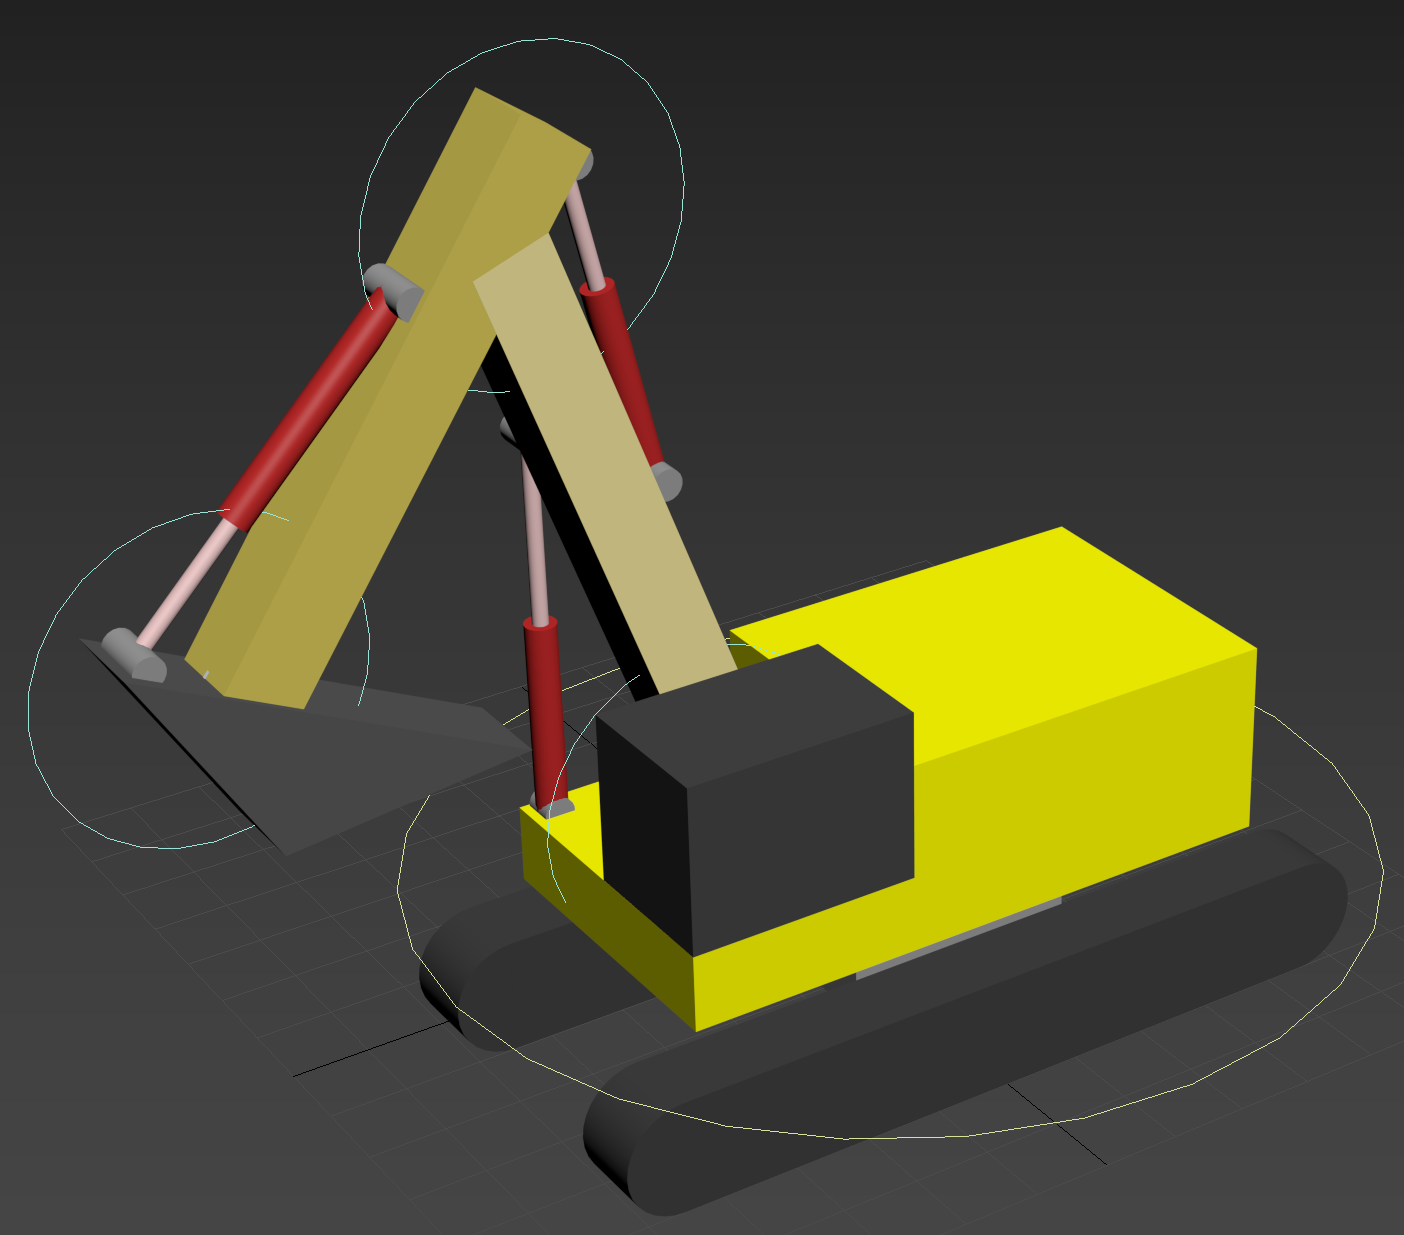
\includegraphics[width=0.5\textwidth]{imagenes/excavadora.png}
   \caption{Modelo final de la excavadora.}
\end{figure}

En las siguientes secciones explicaré el proceso de creación del modelo:
\section{Interpolación cuadrática}

En la práctica se pide implementar la interpolación cuadrática para hacer que los saltos de una plataforma a otra sigan una parábola. A diferencia de la interpolación lineal, esta requiere usar un punto adicional, que es un punto intermedio.

\bigskip

Hay varias formas de realizar la interpolación cuadrática: la más famosa es la interpolación de Lagrange, que para grado 2 es fácil de calcular. Otra opción es utilizar la fórmula de las curvas Bézier para obtener la parábola.

\bigskip

He optado por utilizar la segunda opción porque parecía más fácil de implementar, ya que teníamos la interpolación lineal ya programada. Por tanto, los puntos pasan a ser puntos de control, que al ser unidos se obtienen dos segmentos. A dichos segmentos hay que aplicarles la interpolación lineal con el mismo factor, obteniéndose así dos puntos que forman otro segmento, al que a su vez hay que aplicarle interpolación lineal con el mismo factor que antes. Realizando esto todas las veces que sea necesario, se obtiene una parábola.

\bigskip

Cabe destacar que el objeto no pasará por el punto intermedio, ya que es un punto de control por el que no puede pasar, pero si pasará por el punto de inicio y el final.

% imagen de la animacion esa de wikipedia
\begin{figure}[H]
   \centering
   \includegraphics[width=0.7\textwidth]{imagenes/Bézier_2_big.png}
   \caption{Visualización de la interpolación realizada con un factor de interpolación de 0,7\cite{enwiki:1153684109}.}
\end{figure}

\begin{figure}[H]
    \centering
    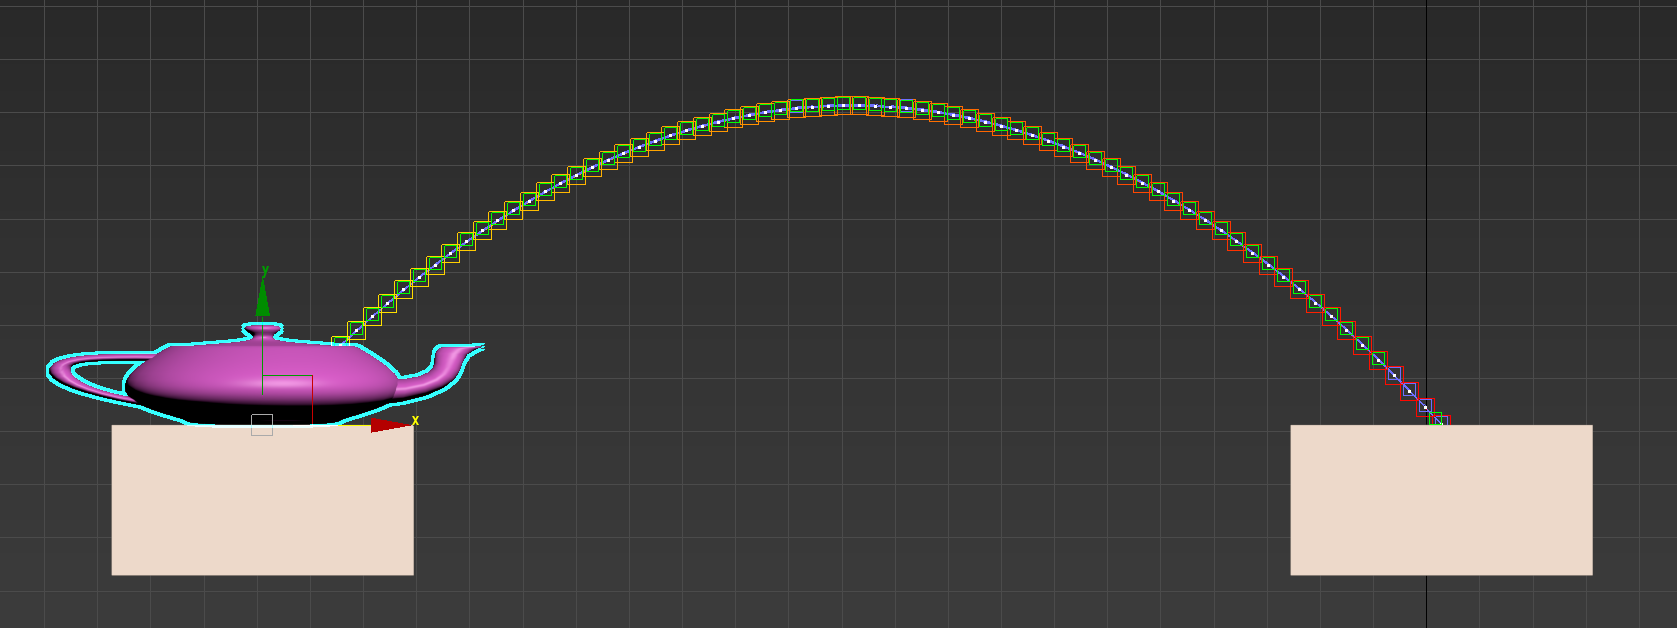
\includegraphics[width=0.8\textwidth]{imagenes/motion path.png}
    \caption{Trayectoria resultante entre dos plataformas con la misma altura.}
 \end{figure}
\section{Interfaz}

La interfaz es la siguiente:

\begin{figure}[H]
   \centering
   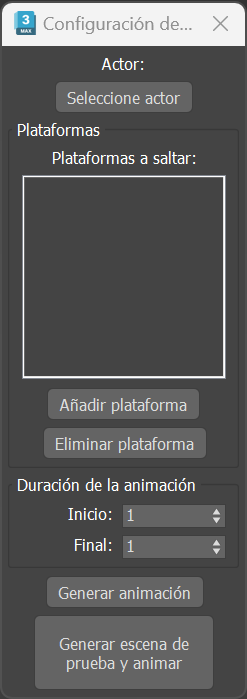
\includegraphics[width=0.2\textwidth]{imagenes/ui1.png}
   \caption{Interfaz del programa.}
\end{figure}

Como se puede ver, aparece un primer botón para elegir el objeto que será animado.

\bigskip

A continuación aparece una lista, junto a dos botones para añadir plataformas o eliminarlas. Conforme se van añadiendo, la lista va creciendo. Además, si se pulsa sobre una de las plataformas de la lista y se le da al botón de eliminar, desaparece de la lista y no se tendrá en cuenta en la animación.

\bigskip

Después, aparece la parte del \textit{timeline}, donde se puede elegir el instante de inicio y de finalización de la animación.

\bigskip

Finalmente aparece el botón de generar la animación, que solo se ejecutará si todo está correctamente elegido.

\bigskip

Como he dicho antes, para asegurarme de que todo esté bien configurado he añadido comprobaciones para no poder elegir el mismo objeto como el que vaya a saltar y como plataforma. Asimismo, he puesto otras como: comprobación de que haya al menos dos plataformas, comprobación de que el tiempo de inicio sea menor que el de finalización y comprobación de que se ha elegido un objeto para animar.

\bigskip
\newpage

A continuación muestro algunos errores que pueden salir:

\begin{figure}[H]
\begin{subfigure}[t]{0.48\textwidth}
    \centering
    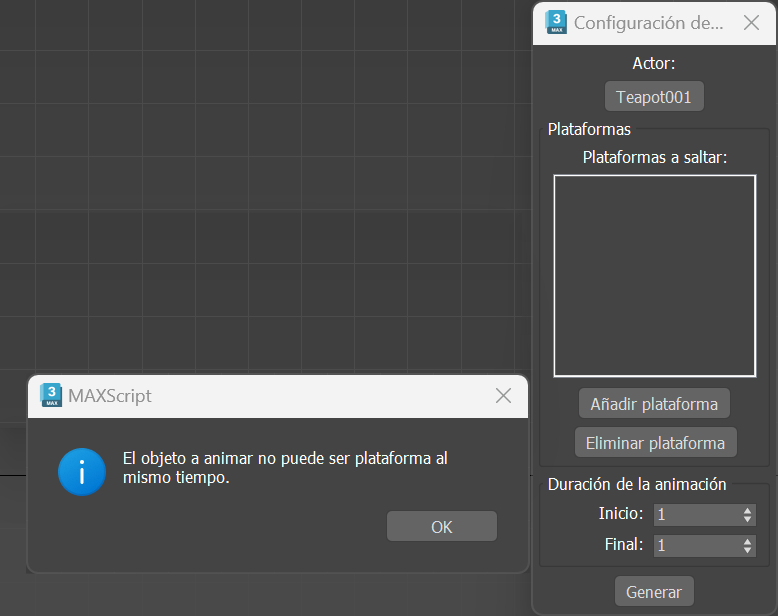
\includegraphics[width=\textwidth]{imagenes/error1.png}
    \caption{Error de un mismo objeto como actor y plataforma.}
 \end{subfigure}
\hfill
 \begin{subfigure}[t]{0.48\textwidth}
    \centering
    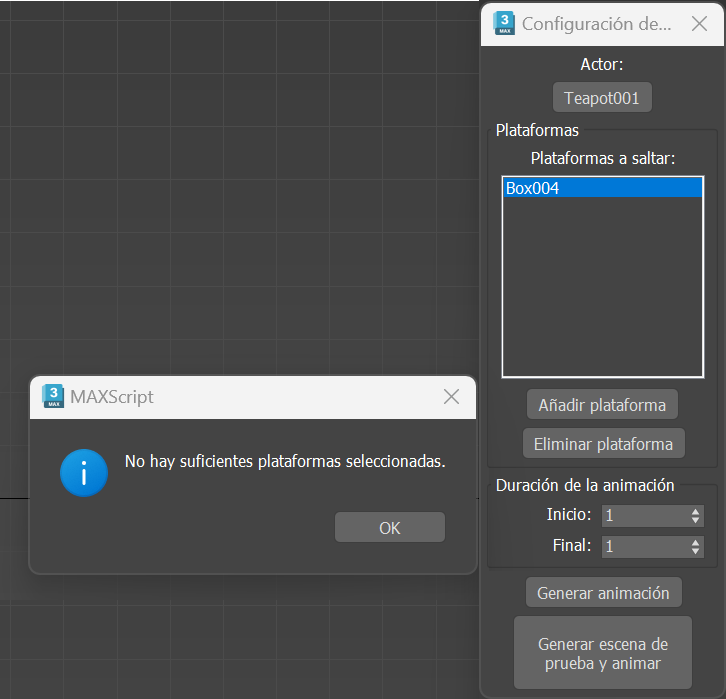
\includegraphics[width=\textwidth]{imagenes/error2.png}
    \caption{Error de no haber suficientes plataformas.}
 \end{subfigure}
\par\bigskip
\begin{subfigure}[t]{\textwidth}
    \centering
    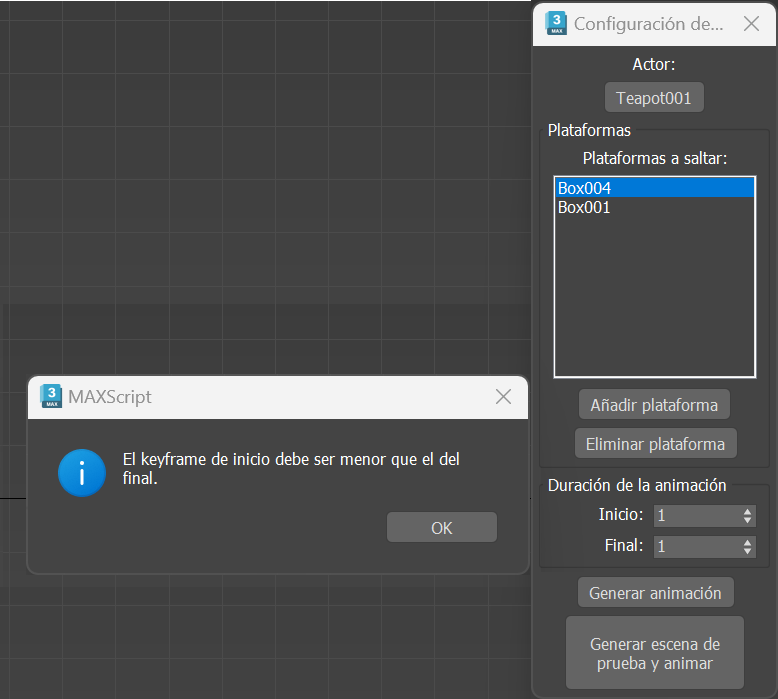
\includegraphics[width=0.48\textwidth]{imagenes/error3.png}
    \caption{Error de intervalo de animación inválido.}
 \end{subfigure}
 \caption{Pantallas con los distintos avisos que puede dar el programa.}
\end{figure}

\newpage

Y un ejemplo de configuración correcta de la interfaz es:

% imagen de la interfaz rellena

\begin{figure}[H]
    \centering
    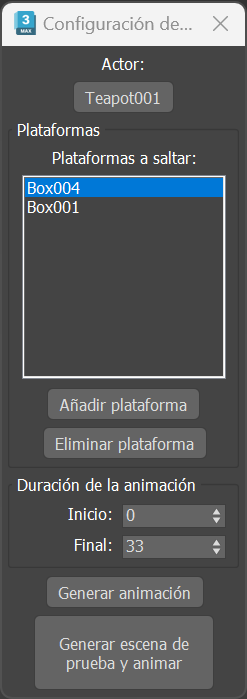
\includegraphics[width=0.2\textwidth]{imagenes/ui2.png}
    \caption{Interfaz con los datos rellenos correctamente.}
 \end{figure}
\section{Animación}

En la animación final, se puede ver como tiene el modificador \textit{Stretch} para simular el aplastamiento y el estiramiento del objeto en movimiento. 

% imagen de esto primero

En cuanto al número de plataformas que puede saltar, es un número arbitrario, mayor o igual a 2, por lo que se pueden poner tantas plataformas como se desee, teniendo en cuenta que al aumentar dicho número la velocidad de la animación aumentará, debido a que tendrá que hacer más cosas en el mismo tiempo.

\bigskip

El punto más alto de cada salto se escoge buscando aquella plataforma que se encuentre más alta y se le suma 80 para que pase por encima de ambas.

\bigskip

Sobre el número de saltos arbitrarios, he necesitado coger las plataformas en pares, de forma que se anime de la plataforma \verb|i| a la plataforma \verb|i+1|, así hasta llegar al final. Cabe destacar que es necesario dividir el número de fotogramas disponibles de manera equitativa, para que los diversos saltos tengan la misma cantidad de tiempo en la animación.

\bigskip

Además, he tenido en cuenta que las plataformas no se encuentren en el suelo o se encuentren escaladas, de forma que la animación resultante siga funcionando.

\bigskip

También he tenido que recortar el \textit{timeline} debido a que si se escogía un valor de inicio distinto de 0, siempre se seguía poniendo ese \textit{keyframe}, haciendo que la animación no fuera correcta hasta llegar al punto de inicio configurado.
\section{Modificador}

El modificador que he utilizado ha sido el de \textit{Stretch}, muy similar a como el ejemplo del seminario, pero algo más refinado.

\bigskip

Este modificador lo que hace en la animación es aplastar el objeto cuando entra en contacto con el suelo y estirarse cuando se encuentra subiendo en el aire. Así se consigue dar la sensación de elasticidad en el objeto.

% foto de las diferencias entre aplastado y estirado
\begin{figure}[H]
    \centering 
	\begin{subfigure}[t]{0.45\textwidth}
	    \centering
	    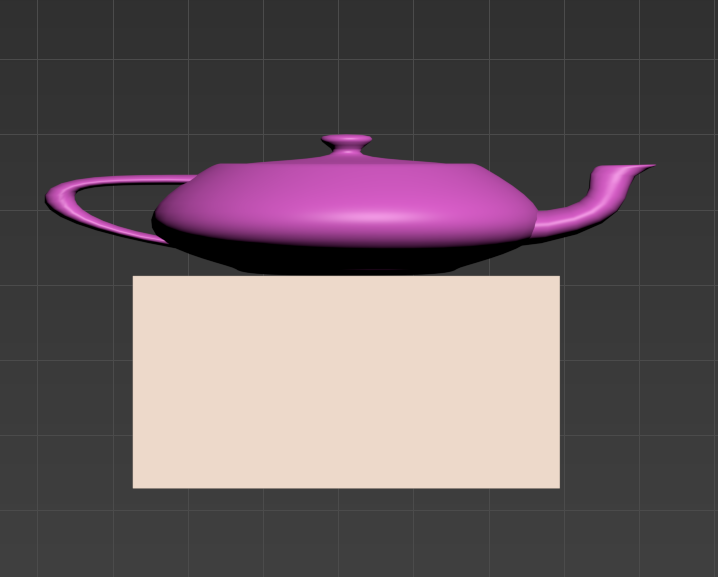
\includegraphics[width=\textwidth]{imagenes/aplastado.png}
        \caption{Objeto aplastado al máximo.}
    \end{subfigure}
    \hfill
	\begin{subfigure}[t]{0.45\textwidth}
	    \centering
	    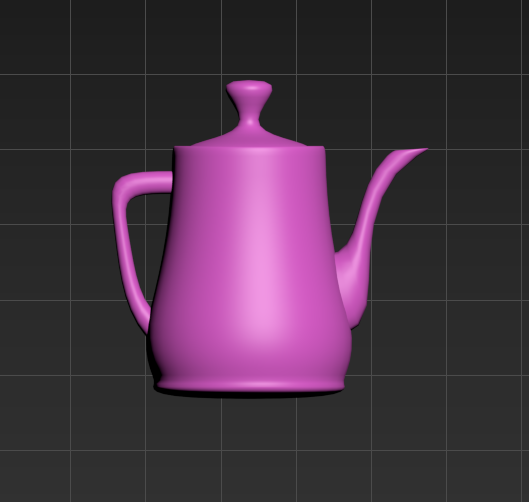
\includegraphics[width=\textwidth]{imagenes/estirado.png}
        \caption{Objeto estirado al máximo.}
    \end{subfigure}    
    \caption{Distintas formas aplicadas por el modificador.}
\end{figure}

Para implementarlo, he hecho que el objeto cuando comienza a subir, hasta llegar a un 15\% en la parábola interpolada, pase de estar aplastado a estirado completamente. Mientras que en los últimos 15\% de la parábola en la bajada, pasa de estar estirado completamente a aplastarse.

\bigskip

He necesitado realizar una interpolación lineal de los valores que toma el modificador \textit{Stretch} para que la animación sea fluida. La fórmula es: $f(t)=(1-t) \cdot ini + t \cdot fin$, donde ``ini'' representa la cantidad de estiramiento que presenta el objeto al inicio y ``fin'' representa la cantidad de estiramiento que presenta el objeto al final.

\bigskip

Además, al tener que realizarse la animación de estiramiento en el intervalo de interpolación [0, 0.15] y para aplastarse en el intervalo [0.85, 1], he necesitado mapear estos valores al intervalo [0, 1], para que el estiramiento y aplastamiento funcionen bien. Para ello, he creado una función \textit{Map Range Clamped}, con el mismo funcionamiento que la función con el mismo nombre en \textit{Unreal Engine}. Además, al ser \textit{clamped} permite que los valores nunca se saldrán del rango al ser evaluados por la función mapeadora.


\end{document}
